We can exactly represent the stack in the $\CESKstart$ machine with a modified allocation scheme for stacks.
%
The key idea is that if the address is ``precise enough,'' then every path that leads to the allocation will proceed exactly the same way until the address is dereferenced.
%

%
\paragraph{``Precise enough'':}
%
For the $\CESKstart$ machine, every function evaluates the same way, regardless of the stack.
%
We should then represent the stack addresses as the components of a function call.
%
The one place in the $\CESKstart$ machine that continuations are allocated is at $\sapp{\mexpri0}{\mexpri1}$ evaluation.
%
The expression itself, the environment, the store and the timestamp are necessary components for evaluating $\sapp{\mexpri0}{\mexpri1}$, so then we just represent the stack address as those four things.
%
The stack is not relevant for its evaluation, so we do not want to store the stack addresses in the same store -- that would also lead to a recursive heap structure.
%
We will call this new table $\mktab$, because it looks like a stack.
%

%
By not storing the continuations in the value store, we separate ``relevant'' components from ``irrelevant'' components.
%
We split the stack store from the value store and use only the value store in stack addresses.
%
Stack addresses generally describe the relevant context that lead to their allocation, so we will refer to them henceforth as \emph{contexts}.
%
The resulting state space is updated here:
  \begin{align*}
    \sa{State} &= \sa{CESK}_t \times \KStore \\
    \Storeable &= \Value \\
    \mkont \in \Kont &::= \epsilon \alt \kcons{\mkframe}{\mctx} \\
    \mctx \in \Context &::=  \tpl{\mexpr,\menv,\mstore}_\mtime \\
    \mktab \in \KStore &= \Context \finto \wp(\Kont) \\
  \end{align*}

The semantics is modified slightly in \autoref{fig:ceskkstart-semantics} to use $\mktab$ instead of $\mstore$ for continuation allocation and lookup.
%
Given finite allocation, contexts are drawn from a finite space, but are still precise enough to describe an unbounded stack: they hold all the relevant components to find which stacks are possible.
%
The computed $\stepto$ relation thus represents the full description of a pushdown system of reachable states (and the set of paths).
%
Of course this semantics does not always define a pushdown system since $\alloc$ can have an unbounded codomain.
%
The correctness claim\ifntr{\footnote{All theorems and proofs are deferred to the extended version available on \url{arXiv.org}.}} is therefore a correspondence between the same machine but with an unbounded stack, no $\mktab$, and $\alloc, \tick$ functions that behave the same disregarding the different representations (a reasonable assumption).
%
\ifntr{See the extended paper for details.}

\begin{figure}
  \centering
  $\mastate,\mktab \stepto \mastate',\mktab'$ \quad $\maddr = \alloc(\mastate,\mktab)$ \quad $\mtimealt = \tick(\mastate,\mktab)$ \\
  \begin{tabular}{r|l}
    \hline\vspace{-3mm}\\
    $\tpl{\svar\mvar, \menv, \mstore, \makont}_\mtime,\mktab$
    &
    $\tpl{\mval, \mstore,\makont}_\mtimealt,\mktab$ if $\mval \in \mstore(\menv(\mvar))$
    \\
% Application
    $\tpl{\sapp{\mexpri0}{\mexpri1},\menv,\mstore,\makont}_\mtime,\mktab$
    &
    $\tpl{\mexpri0,\menv,\mstore,\kcons{\appl{\mexpri1,\menv}}{\mctx}}_\mtimealt,\mktab'$ \\
    where & $\mctx = \tpl{\sapp{\mexpri0}{\mexpri1},\menv,\mstore}_\mtime$ \\
          & $\mktab' = \joinm{\mktab}{\mctx}{\makont}$
    \\
% Arg eval
    $\tpl{\mval,\mstore,\kcons{\appl{\mexpr,\menv'}}{\mctx}}_\mtime,\mktab$
    &
    $\tpl{\mexpr,\menv',\mstore,\kcons{\appr{\mval}}{\mctx}}_\mtimealt,\mktab$
    \\
% Function call
    $\tpl{\mval,\menv,\mstore,\kcons{\appr{\slam{\mvar}{\mexpr},\menv'}}{\mctx}}_\mtime,\mktab$
    &
    $\tpl{\mexpr,\menv'',\mstore',\makont}_\mtimealt,\mktab$ if $\makont \in \mktab(\mctx)$ \\
    where & $\menv'' = \extm{\menv'}{\mvar}{\maddr}$ \\
          & $\mstore' = \joinm{\mstore}{\maddr}{\mval}$
  \end{tabular}
  \caption{$\CESKKstart$ semantics}
  \label{fig:ceskkstart-semantics}
\end{figure}

\iftr{
\subsection{Correctness}

The high level argument for correctness exploits properties of both machines.
%
Where the stack is unbounded (call this $\CESKt$), if every state in a trace shares a common tail in their continuations, that tail is \emph{irrelevant}.
%
This means the tail can be replaced with anything and still produce a valid trace.
%
We call this property more generally, ``context irrelevance.''
%
The $\CESKKstart$ machine maintains an invariant on $\mktab$ that says that $\makont \in \mktab(\mctx)$ represents a trace in $\CESKt$ that starts at the base of $\makont$ and reaches $\mctx$ with $\makont$ on top.
%
We can use this invariant and context irrelevance to translate steps in the $\CESKKstart$ machine into steps in $\CESKt$.
%
The other way around, we use a proposition that a full stack is represented by $\mktab$ via unrolling and follow a simple simulation argument.

The common tail proposition we will call $\hastail$ and the replacement function we will call $\replacetail$; they both have obvious inductive and recursive definitions respectively.
%
The invariant is stated with respect to the entire program, $\mexpr_\mathit{pgm}$:
\begin{mathpar}
  \inferrule{ }{\invmktab(\bot)} \quad
  \inferrule{\invmktab(\mktab) \\
      \forall \makont_c \in K. \startstate(\makont_c) \stepto_\CESKt^* \tpl{\mexpr_c,\menv_c,\mstore_c,\append{\mkont_c}{\epsilon}}_{\mtime_c}}
            {\invmktab(\extm{\mktab}{\tpl{\mexpr_c,\menv_c,\mstore_c}_{\mtime_c}}{K})} \\

  \inferrule{
    % invariant for current state
    \startstate(\makont) \stepto_\CESKt^* \tpl{\mexpr,\menv,\mstore,\append{\makont}{\epsilon}}_\mtime \\
    % invariant for all entries
    \invmktab(\mktab)}
    {\inv(\tpl{\mexpr,\menv,\mstore,\makont}_\mtime,\mktab)}
  \end{mathpar}
where
\begin{align*}
 \startstate(\epsilon) &= \tpl{\mexpr_\mathit{pgm},\bot,\bot,\epsilon}_{\mtime_0} \\
                \startstate(\kcons{\mkframe}{\tpl{\mexpr_c,\menv_c,\mstore_c}_{\mtime_c}}) &=
                \tpl{\mexpr_c,\menv_c,\mstore_c,\epsilon}_{\mtime_c}
\end{align*}
We use $\append{\cdot}{\epsilon}$ to treat $\mctx$ like $\epsilon$ and construct a continuation in $\Kont$ rather than $\sa{Kont}$.
%%
\begin{lemma}[Context irrelevance]\label{lem:irrelevance}
  For all traces $\mtrace \in \CESKt^*$ and continuations $\mkont$ such that $\hastail(\mtrace,\mkont)$, for any $\mkont'$, $\replacetail(\mtrace,\mkont,\mkont')$ is a valid trace.
\end{lemma}
\begin{proof}
  Simple induction on $\mtrace$ and cases on $\stepto_{\CESKt}$.
\end{proof}
\begin{lemma}[$\CESKKstart$ Invariant]\label{lem:invariant}
  For all $\mstate,\mstate' \in \sa{State}$, if $\inv(\mstate)$ and $\mstate \stepto \mstate'$, then $\inv(\mstate')$
\end{lemma}
\begin{proof}
  Routine case analysis.
\end{proof}
Note that the injection of $\mexpr_\mathit{pgm}$ into $\CESKKstart$, $(\tpl{\mexpr_\mathit{pgm},\bot,\bot,\epsilon}_{\mtime_0},\bot)$, trivially satisfies $\inv$.

The unrolling proposition is the following
\begin{mathpar}
  \inferrule{ }{\epsilon \in \unroll{\mktab}{\epsilon}} \quad
  \inferrule{\makont \in \mktab(\mctx),
             \mkont \in \unroll{\mktab}{\makont}}
            {\kcons{\mkframe}{\mkont} \in \unroll{\mktab}{\kcons{\mkframe}{\mctx}}}
\end{mathpar}
\begin{theorem}[Correctness]\label{thm:pushdown-correct}
  For all expressions $\mexpr_\mathit{pgm}$,
  \begin{itemize}
  \item{{\bf Soundness: } %for all $\mstate\equiv\tpl{\mexpr,\menv,\mkont},\mstate'\equiv{\mexpr',\menv',\mkont'} \in \CESKt$,
        if $\mstate \stepto_{\CESKt} \mstate'$,
        %for all $\mktab,\makont$ if
        $\inv(\mstate\set{\mkont := \makont},\mktab)$,
        and $\mkont \in \unroll{\mktab}{\makont}$, then
        there are $\mktab',\makont'$ such that
        $\mstate\set{\mkont := \makont},\mktab \stepto_{\CESKKstart} \mstate'\set{\mkont := \makont'},\mktab'$ and $\mkont' \in \unroll{\mktab'}{\makont'}$}
  \item{{\bf Completeness:} if $\mastate,\mktab \stepto_{\CESKKstart} \mastate',\mktab'$
      and $\inv(\mastate,\mktab)$,
      for all $\mkont$, if $\mkont \in \unroll{\mktab}{\mastate.\makont}$ then
      there is a $\mkont'$ such that
      $\mastate\set{\makont := \mkont} \stepto_{\CESKt}
       \mastate'\set{\makont := \mkont'}$ and
       $\mkont' \in \unroll{\mktab}{\mastate'.\makont}$.}
  \end{itemize}
\end{theorem}
}

\paragraph{Revisiting the example}

First we consider what \zcfa{} gives us, to see where pushdown analysis improves.
%
The important difference is that in \kcfa{}, return points are stored in an address that is linked to the textual location of the function call, plus a $k$-bounded amount of calling history.
%
So, considering the common $k = 0$, the unknown function call within map (either \texttt{render{-}int} or \texttt{fact}) returns from the context of the second call to \texttt{map} to the context of the first call to \texttt{map}.
%
Non-tail calls aren't safe from imprecise return flow: the recursive call to \texttt{map} returns directly to both calls in the outer \texttt{cons}.
%
All nonsense.
%
Control-flow graphs from \zcfa{} read like a 3-year-old's scribblings.
%

In our presentation, return points are stored in an address that represents the \emph{exact} calling context with respect to the abstract machine's components.
%
This means when there is a ``merging'' of return points, it really means that two places in the program have requested the exact same thing of a function, even with the same global values.
%
The function \emph{will} return to both places.
%
The predicted control flow in the example is as one would expect, or \emph{hope}, an analysis would predict: the correct flow.

\subsection{Engineered semantics for efficiency}\label{sec:eng-frontier}
%%
We cover three optimizations that may be employed to accelerate the fixed-point computation.
\begin{enumerate}
\item{\label{item:chunk}Continuations can be ``chunked'' more coarsely at function boundaries instead of at each frame in order to minimize table lookups.}
\item{We can globalize $\mktab$ with no loss in precision, unlike a global store;%
      it will not need to be stored in the frontier but will need to be tracked by seen states.
%
      The seen states only need comparison, and a global $\mktab$ increases monotonically, so we can use Shivers' timestamp technique~\citep{ianjohnson:Shivers:1991:CFA}.
%
      The timestamp technique does not store an entire $\mktab$ in the seen set at each state, but rather how many times the global $\mktab$ has increased.}
\item{Since evaluation is the same regardless of the stack, we can memoize results to short-circuit to the answer.
      The irrelevance of the stack then precludes the need for timestamping the global $\mktab$.}
\end{enumerate}
%
This last optimization will be covered in more detail in \autoref{sec:memo}.
%
From here on, this paper will not explicitly mention timestamps.

A secondary motivation for the representation change in \ref{item:chunk} is that flow analyses commonly split control-flow graphs at function call boundaries to enable the combination of intra- and inter-procedural analyses.
%
In an abstract machine, this split looks like installing a continuation prompt at function calls.
%
We borrow a representation from literature on delimited continuations~\citep{ianjohnson:Biernacki2006274} to split the continuation into two components: the continuation and meta-continuation.
%
Our delimiters are special since each continuation ``chunk'' until the next prompt has bounded length.
%
The bound is roughly the deepest nesting depth of an expression in functions' bodies.
%
Instead of ``continuation'' and ``meta-continuation'' then, we will use terminology from CFA2 and call the top chunk a ``local continuation,'' and the rest the ``continuation.''\footnote{Since the continuation is either $\epsilon$ or a context, CFA2 calls these ``entries'' to mean execution entry into the program ($\epsilon$) or a function ($\mctx$). One can also understand these as entries in a table ($\mktab$). We stay with the ``continuation'' nomenclature because they represent full continuations.}
%
%

\autoref{fig:pushdown-vis} has a visualization of a hypothetical state space.
%
Reduction relations can be thought of as graphs: each state is a node, and if a state $\mstate$ reduces to $\mstate'$, then there is an edge $\mstate \stepto \mstate'$.
%
We can also view our various environments that contain pointers (addresses, contexts) as graphs: each pointer is a node, and if the pointer $\mctx$ references an object $\mlkont$ that contains another pointer $\mctx'$, then there is a labeled edge $\mctx \xrightarrow{\mlkont} \mctx'$.
%
States' contexts point into $\mktab$ to associate each state with a \emph{regular language} of continuations.
%
The reversed $\mktab$ graph can be read as a group of finite state machines that accepts all the continuations that are possible at each state that the reversed pointers lead to.
%
The $\kmt$ continuation is this graph's starting state.

\begin{figure}
  \centering
  \begin{tabular}{rlrl}
    $\mastate \in \sa{CESIK}$ &\hspace{-3mm}$= \tpl{\mexpr,\menv,\mstore,\mlkont,\makont}$& $\mlkont \in \LKont$ &\hspace{-3mm}$= \Frame^*$ \\
    & & $\makont \in \Kont$ &\hspace{-3mm}$::= \epsilon \alt \mctx$
  \end{tabular}
  \caption{$\CESIKKstar$ semantic spaces}
  \label{fig:pushdown-spaces}
\end{figure}

\begin{figure}
  \centering
  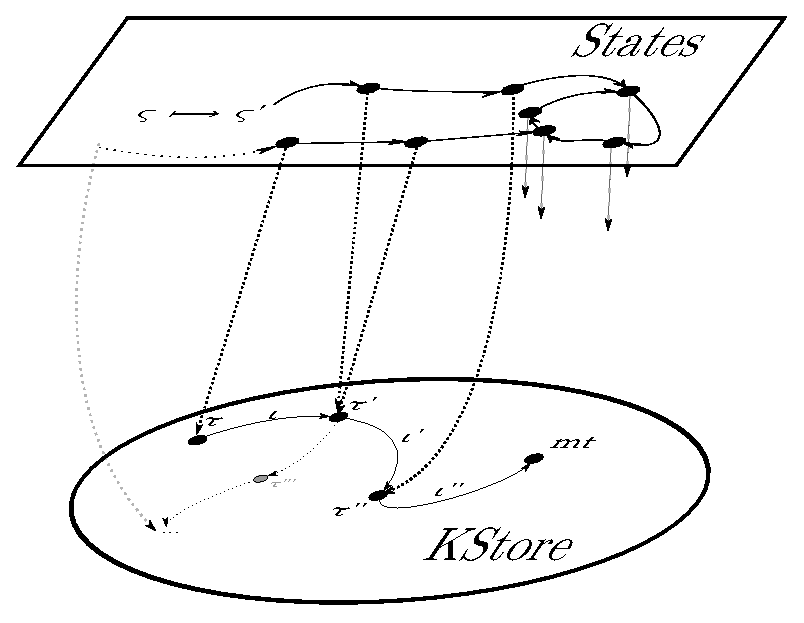
\includegraphics[scale=0.65]{xigraph-cloud}
  \caption{Graph visualization of states and $\mktab$}
  \label{fig:pushdown-vis}
\end{figure}

The resulting shuffling of the semantics to accommodate this new representation is in \autoref{fig:cesikkstar-semantics}.
%
The extension to $\mktab$ happens in a different rule -- function entry -- so the shape of the context changes to hold the function, argument, and store.
%
We have a choice of whether to introduce an administrative step to dereference $\mktab$ once $\mlkont$ is empty, or to use a helper metafunction to describe a ``pop'' of both $\mlkont$ and $\mkont$.
%
Suppose we choose the second because the resulting semantics has a 1-to-1 correspondence with the previous semantics.
%
A first attempt might land us here:
\begin{align*}
  \pop(\kcons{\mkframe}{\mlkont},\makont,\mktab) &= \set{(\mkframe,\mlkont,\makont)} \\
  \pop(\epsilon,\mctx,\mktab) &= \setbuild{(\mkframe,\mlkont,\makont)}{(\kcons{\mkframe}{\mlkont}, \makont) \in \mktab(\mctx)}
\end{align*}
However, tail calls make the dereferenced $\mctx$ lead to $(\epsilon,\mctx')$.
%
Because abstraction makes the store grow monotonically in a finite space, it's possible that $\mctx' = \mctx$ and a naive recursive definition of $\pop$ will diverge chasing these contexts.
%
Now $\pop$ must save all the contexts it dereferences in order to guard against divergence.
%
So $\pop(\mlkont,\makont,\mktab) = \popaux(\mlkont,\makont,\mktab,\emptyset)$ where
\begin{align*}
  \popaux(\epsilon,\epsilon,\mktab,G) &= \emptyset \\
  \popaux(\kcons{\mkframe}{\mlkont},\makont,\mktab,G) &= \set{(\mkframe,\mlkont,\makont)} \\
  \popaux(\epsilon,\mctx,\mktab,G) &= \setbuild{(\mkframe,\mlkont,\makont)}{(\kcons{\mkframe}{\mlkont}, \makont) \in \mktab(\mctx)} \\
  &\cup \bigcup\limits_{\mctx' \in G'}\popaux(\epsilon,\mctx',\mktab,G\cup G') \\
  \text{where } G' &= \setbuild{\mctx'}{(\epsilon,\mctx') \in \mktab(\mctx)} \setminus G
\end{align*}

In practice, one would not expect $G$ to grow very large.
%
Had we chosen the first strategy, the issue of divergence is delegated to the machinery from the fixed-point computation.\footnote{CFA2 employs the first strategy and calls it ``transitive summaries.''}
%
However, when adding the administrative state, the ``seen'' check requires searching a far larger set than we would expect $G$ to be.

\begin{figure}
  \centering
  $\mastate,\mktab \stepto \mastate',\mktab'$ \quad $\maddr = \alloc(\mastate,\mktab)$ \\
  \begin{tabular}{r|l}
    \hline\vspace{-3mm}\\
    $\tpl{\svar\mvar, \menv, \mstore, \mlkont, \makont},\mktab$
    &
    $\tpl{\mval,\mstore,\mlkont,\makont},\mktab$ if $\mval \in \mstore(\menv(\mvar))$
    \\
% Application
    $\tpl{\sapp{\mexpri0}{\mexpri1},\menv,\mstore,\mlkont,\makont},\mktab$
    &
    $\tpl{\mexpri0,\menv,\mstore,\kcons{\appl{\mexpri1,\menv}}{\mlkont},\makont},\mktab$
    \\
% Arg eval
    $\tpl{\mval, \mstore, \mlkont,\makont},\mktab$
    &
    $\tpl{\mexpr,\menv',\mstore,\kcons{\appr{\mval,\menv}}{\mlkont'},\makont'},\mktab$ \\
    &
    if $\appl{\mexpr,\menv'},\mlkont',\makont' \in \pop(\mlkont,\makont,\mktab)$ \\
% Function call
    $\tpl{\mval,\mstore, \mlkont,\makont},\mktab$
    &
    $\tpl{\mexpr,\extm{\menv}{\mvar}{\maddr},\mstore',\epsilon,\mctx},\mktab'$ \\
    & if $\appr{\slam{\mvar}{\mexpr},\menv}, \mlkont', \makont' \in \pop(\mlkont,\makont,\mktab)$ \\
    where & $\mstore' = \joinm{\mstore}{\maddr}{\mval}$ \\
    & $\mctx = (\tpl{\slam{\mvar}{\mexpr},\menv},\mval,\mstore)$ \\
    & $\mktab' = \joinm{\mktab}{\mctx}{(\mlkont,\makont)}$
  \end{tabular} \\
  \caption{$\CESIKKstar$ semantics}
  \label{fig:cesikkstar-semantics}
\end{figure}

\begin{align*}
  {\mathcal F}_{\mexpr}(S,R,F,\mktab) &= (S \cup F, R \cup R', F'\setminus S, \mktab') \\
  I &= \bigcup\limits_{s=(\mastate,\mstore) \in F}{\setbuild{(\tpl{\mastate,\mastate'}, \mktab')}{\mastate,\mktab \stepto \mastate',\mktab'}} \\
  R' &= \pi_0 I \qquad F' = \pi_1 R' \qquad \mktab' = \bigsqcup\pi_1 I
\end{align*}
For a program $\mexpr$, we will say $(\emptyset,\emptyset,\set{\tpl{\mexpr,\bot,\bot,\epsilon,\epsilon}},\bot)$ is the bottom element of ${\mathcal F}_{\mexpr}$'s domain.
%
The ``analysis'' then is then the pair of the $R$ and $\mktab$ components of $\lfp({\mathcal F}_{\mexpr})$.

\iftr{
\paragraph{Correctness} The correctness argument for this semantics is not about single steps but instead about the entire relation that ${\mathcal F}$ computes.
%
The argument is that the $R$ and $\mktab$ components of the system represent a slice of the unbounded relation $\stepto_{\CESK}$ (restricted to reachable states).
%
We will show that traces in any $n \in \nat$ times we \emph{unfold} $\stepto_{\CESK}$ from the initial state, there is a corresponding $m$ applications of ${\mathcal F}$ that reify into a relation that exhibit the same trace.
%
Conversely, any trace in the reification of ${\mathcal F}_{\mexpr}^m(\bot)$ has the same trace in some $n$ unfoldings of $\stepto_{\CESK}$.
%
For an arbitrary $\alloc$ function, we cannot expect ${\mathcal F}$ to have a fixed point, so this property is the best we can get.
%
For a finite $\alloc$ function, Kleene's fixed point theorem dictates there is a $m$ such that ${\mathcal F}_{\mexpr}^m(\bot)$ is a fixed point, so every trace in the reified relation is also a trace in an unbounded number of unfoldings of $\stepto_{\CESK}$.
%
This is the corresponding completeness argument for the algorithm.

\begin{align*}
  \reachrestrict(\mstate_0, \stepto, 0) &= \setbuild{(\mstate_0,\mstate)}{\mstate_0 \stepto \mstate} \\
  \reachrestrict(\mstate_0, \stepto, n+1) &= \stepextend(\reachrestrict(\mstate_0,\stepto,n)) \\
  \textit{where } \stepextend(R) &= R \cup \setbuild{(\mstate,\mstate')}{(\_,\mstate) \in R, \mstate \stepto \mstate'}
\end{align*}
The reification simply realizes all possible complete continuations that a state could have, given $\mktab$:
\begin{mathpar}
  \inferrule{
  \tpl{\tpl{\mexpr,\menv,\mstore,\makont},
      \tpl{\mexpr',\menv',\mstore',\makont'}} \in R \\
  \mkont \in \tails{\mktab}{\makont}}
  {\tpl{\mexpr,\menv,\mstore,\append{\makont}{\mkont}} \stepto_{\reify(S,R,F,\mktab)}
   \tpl{\mexpr',\menv',\mstore'\append{\makont'}{\mkont}}}
  % \reify(S,F,R,\mktab) &= \setbuild{}
  % {\\ &\phantom{= \{}
  %   \tpl{(\tpl{\mexpr,\menv,\makont},\mstore,\mtime),
  %     (\tpl{\mexpr',\menv',\makont'},\mstore',\mtime')} \in R,
  %   \\ &\phantom{= \{}
  %   \mkont \in \tails{\mktab}{\makont}}
\end{mathpar}
The additional judgment about tails is a variant of $\mathit{unroll}$ in order to get a common tail:
\begin{mathpar}
  \inferrule{ }{\epsilon \in \tails{\mktab}{\epsilon}} \quad
  \inferrule{\makont \in \mktab(\mctx) \\
             \mkont \in \unroll{\mktab}{\makont}}
            {\mkont \in \tails{\mktab}{\kcons{\mkframe}{\mctx}}}
\end{mathpar}
\begin{theorem}[Correctness]\label{thm:global-pushdown}
  For all $\mexpr_0$, let $\mstate_0 = \tpl{\mexpr_0,\bot,\bot,\epsilon}$ in
  $\forall n \in \nat, \mstate,\mstate' \in \CESK$:
  \begin{itemize}
  \item{if $(\mstate,\mstate') \in \reachrestrict(\mstate_0,\stepto_{\CESK},n)$ then
      there is an $m$ such that $\mstate \stepto_{\reify({\mathcal F}_{\mexpr_0}^m(\bot))} \mstate'$}
  \item{if $\mstate \stepto_{\reify({\mathcal F}_{\mexpr_0}^n(\bot))} \mstate'$ then
      there is an $m$ such that $(\mstate,\mstate') \in \reachrestrict(\mstate_0,\stepto_{\CESK},m)$}
  \end{itemize}
\end{theorem}
\begin{proof}
  By induction on $n$.
\end{proof}
}

\subsection{Remarks about cost}

The common tradeoff for performance over precision is to use a global store.
%
A representation win originally exploited by Shivers~\citep{ianjohnson:Shivers:1991:CFA} is to represent the seen states' stores by the \emph{age} of the store.
%
A context in this case contains the store age for faster comparison.
%
Old stores are mostly useless since the current one subsumes them, so a useful representation for the seen set is as a map from the \emph{rest of the state} to the store age it was last visited with.
%
We will align with the analysis literature and call these ``rest of state'' objects \emph{points}.
%
Note that since the store age becomes part of the state representation due to ``context,'' there are considerably more points than in the comparable finite state approach.
%
When we revisit a state because the store age (or $\mktab$ age) is different from the last time we visited it (hence we're visiting a \emph{new state}), we can clobber the old ages.
%
A finite state approach will use less memory because the seen set will have a smaller domain (fewer distinctions made because of the lack of a ``context'' component).
%
%Finite state approaches can take less time, but not always: stack-allocation-inspired binding techniques can regain precision and performance.
%
%  LocalWords:  CESK lookup pushdown codomain optimizations chunked
%  LocalWords:  lookups memoize timestamps rlrl reify unfoldings
%  LocalWords:  Kleene's reified reification
